%!TEX root = ../../exa-ma-d7.1.tex
\section{Software: \texorpdfstring{\Feelpp}{Feel++}}
\label{sec:Feelpp:software}

\begin{table}[!ht]
    \centering
    { \setlength{\parindent}{0pt}
    \def\arraystretch{1.25}
    \arrayrulecolor{numpexgray}
    {\fontsize{9}{11}\selectfont
    \begin{tabular}{!{\color{numpexgray}\vrule}p{.4\textwidth}!{\color{numpexgray}\vrule}p{.6\textwidth}!{\color{numpexgray}\vrule}}
        \rowcolor{numpexgray}{\rule{0pt}{2.5ex}\color{white}\bf Field} & {\rule{0pt}{2.5ex}\color{white}\bf Details} \\
        \rowcolor{white}\textbf{Consortium} & \begin{tabular}{l}
\Feelpp Consortium\\
\end{tabular} \\
        \rowcolor{numpexlightergray}\textbf{Exa-MA Partners} & \begin{tabular}{l}
CNRS\\
Inria Grenoble\\
Unistra\\
\end{tabular} \\
        \rowcolor{white}\textbf{Contact Emails} & \begin{tabular}{l}
christophe.prudhomme@cemosis.fr\\
vincent.chabannes@cemosis.fr\\
\end{tabular} \\
        \rowcolor{numpexlightergray}\textbf{Supported Architectures} & \begin{tabular}{l}
CPU Only\\
\end{tabular} \\
        \rowcolor{white}\textbf{Repository} & \href{https://github.com/feelpp/feelpp}{https://github.com/feelpp/feelpp} \\
        \rowcolor{numpexlightergray}\textbf{License} & \begin{tabular}{l}
OSS:: GPL v*\\
OSS:: LGPL v*\\
\end{tabular} \\
        \rowcolor{white}\textbf{Bottlenecks roadmap} & \begin{tabular}{l}
B10 - Scientific Productivity\\
B11 - Reproducibility and Replicability of Computation\\
B12 - Pre/Post Processing and In-Situ Processing\\
B2 - Interconnect Technology\\
B6 - Data Management\\
B7 - Exascale Algorithms\\
\end{tabular} \\
        \hline
    \end{tabular}
    }}
    \caption{\Feelpp Information}
\end{table}

\subsection{Software summary}
\label{sec:Feelpp:summary}

\feelpp is a powerful framework designed to solve problems based on ordinary differential equations (ODEs) and partial differential equations (PDEs).
It leverages modern \Cpp{} standards, including \Cpp{17} and \Cpp{20}, and also provides a Python layer through Pybind11.
The suite is particularly effective for parallel computing, with seamless integration of parallelism through default communicators, including support for ensemble runs.



\Feelpp provides several specialized toolboxes to address various fields of numerical simulation
\begin{inparaenum}[(i)]
        \item fluid mechanics,
        \item solid mechanics,
        \item heat transfer and conjuguate heat transfer,
        \item fluid structure interaction,
        \item electro and magnetostatic,
        \item thermoelectric,
        \item levelset and multifluid.
\end{inparaenum}
Each toolbox is tailored to specific types of problems, ensuring high performance and accuracy.

\Feelpp is used in a variety of fields, particularly in health, industry, and physics. Below are some examples of applications:
\begin{inparaenum}[(i)]
    \item \textbf{Health (Brain)}: Applications related to brain modeling.
    \item \textbf{Health (Tumor Cells)}: Simulation of tumor cell behavior.
    \item \textbf{Industry (ROM, UQ)}: Reduced-order modeling and uncertainty quantification in industrial settings.
    \item \textbf{Automotive (CFD, ROM)}: Computational fluid dynamics and reduced-order models in automotive engineering.
    \item \textbf{Physics (High Field Magnets)}: Simulations of high field magnets.
    \item \textbf{Health (Rheology)}: Modeling blood rheology.
    \item \textbf{Health (Eye/Brain)}: Coupling between the eye and the brain in medical simulations.
\end{inparaenum}

The \Feelpp core library provides a wide range of numerical methods for solving PDEs, with support for finite elements in various Sobolev spaces with scalar, vector and matrix values. For example:
\begin{inparaenum}[(i)]
    \item \( L^2 \), \( \mathbf{L}^2 \), \( \mathbb{L}^2 \)
    \item \( H^1 \), \( \mathbf{H}^1 \), \( \mathbb{H}^1 \)
    \item \( \mathbf{H}(\text{div}) \), \( \mathbf{H}(\text{curl}) \)
\end{inparaenum}

\Feelpp supports a wide variety of element types and value types, including single, double, and quad precision, as well as complex numbers. The supported problem domains include 0D to 3D, with or without time dependence.

Here is a typical example of solving a Laplace equation in \Feelpp:

\begin{listing}[ht]
        \caption{Sample \Feelpp code for solving a Laplace equation on an arbitrary domain.}
\begin{minted}[
        linenos,                % Line numbers
        fontsize=\scriptsize,        % Reduce font size
        bgcolor=bgcolor,        % Slightly gray background
        frame=lines,            % Delimiters around the code
        framesep=2mm,           % Space between code and frame
        rulecolor=\color{gray}, % Color of the frame
        breaklines              % Allow line breaks in long lines
      ]{cpp}
auto Vh = Pch<4>(mesh, markedelements(mesh, expr("<...>")));
auto u = Vh->element(), v = Vh->element(g, "g");
auto l = form1(_test = Vh);
l = integrate(_range = elements(support(Vh)), _expr = f * id(v));
l += integrate(_range = markedfaces(support(Vh), "Robin"), _expr = -r_2 * id(v));
l += integrate(_range = markedfaces(support(Vh), "Neumann"), _expr = -un * id(v));

auto a = form2(_trial = Vh, _test = Vh);
a = integrate(_range = elements(support(Vh)), _expr = inner(k * gradt(u), grad(v)));
a += integrate(_range = markedfaces(support(Vh), "Robin"), _expr = r_1 * idt(u) * id(v));
a += on(_range = markedfaces(support(Vh), "Dirichlet"), _rhs = l, _element = u, _expr = g);
a.solve(_rhs = l, _solution = u);
\end{minted}
\end{listing}

The suite supports multiple linear algebra libraries, including PETSc, SLEPc, Eigen, and Boost::ublas, and is designed to run efficiently in both sequential and parallel environments.



\Feelpp is a versatile and powerful tool for solving PDEs and ODEs in a variety of scientific and industrial applications.
With support for high-performance computing and a broad range of numerical methods which can be used to build taylored applications for research, development, and teaching.


\subsection{Purpose}
\label{sec:Feelpp:purpose}
\Feelpp aims to provide a flexible and efficient environment for conducting finite element analysis in multiple scientific domains.
It allows for the rapid prototyping of numerical models and is built with parallel computing in mind to scale on modern HPC architectures.

\subsection{Programming and Computational Environment}
\label{sec::Feelpp:environment_capabilities}

The~\Cref{tab:Feelpp:environment_capabilities} summarizes these aspects for \Feelpp, providing a view of its programming and computational capabilities.

%% \begin{table}[!ht]
%% %%    \centering
%%     {
%%     \setlength{\parindent}{0pt}
%%     \def\arraystretch{1.25}
%%     \arrayrulecolor{numpexgray}
%%     {\fontsize{9}{11}\selectfont
%%     \begin{longtable}{lp{.3\textwidth}p{.5\textwidth}}
%%         \rowcolor{gray}\textbf{\color{white}Category} & \textbf{\color{white}Details} & \textbf{\color{white}Description} \\
%%         \hline
%%         \endfirsthead % End of the first head (the header for the first page)
%%
%%         \hline
%%         \rowcolor{gray}\textbf{Category} & \textbf{Details} & \textbf{Description} \\
%%         \hline
%%         \endhead % End of the head (for all other pages)
%%
%%         \hline
%%         \endfoot % Footer for all but the last page
%%
%%         \hline
%%         \endlastfoot % Footer for the last page
%%
%%         \rowcolor{white}Languages  & \begin{tabular}{l}
%% C++\\
%% C++17\\
%% C++20\\
%% Python\\
%% \end{tabular} & \Feelpp is primarily developed in C++ and supports modern C++ standards, including C++17 and C++20, which provide enhanced performance, safety features, and modern programming paradigms for high-performance computing applications. This allows \Feelpp to leverage advanced language features such as constexpr, parallel algorithms, and enhanced lambda expressions, improving both code maintainability and computational efficiency. Additionally, \Feelpp integrates with Python, enabling scripting capabilities and facilitating ease of use for rapid prototyping, automation, and integration with scientific workflows. This dual-language support provides flexibility for both performance-critical tasks and user-friendly interfaces. \\
%%         \rowcolor{numpexlightergray}Parallelism  & \begin{tabular}{l}
%% MPI\\
%% Parallelism - C++\\
%% Task based\\
%% \end{tabular} & \Feelpp offers robust support for parallel computing, making it suitable for high-performance simulations. It utilizes MPI (Message Passing Interface) for distributed memory parallelism, enabling efficient communication between processes across different nodes in HPC environments. Additionally, \Feelpp implements parallelism directly in C++, allowing fine-grained control over threading and parallel execution within shared memory systems. The framework also supports task-based parallelism thanks to specx, enabling the efficient execution of independent computational tasks, improving load balancing, and optimizing resource usage across heterogeneous computing architectures. This parallelism support ensures scalability and high performance in complex multiphysics simulations.\\
%%         \rowcolor{white}Data Formats  & \begin{tabular}{l}
%% Data-management system\\
%% Ensight\\
%% Gmsh and associated formats\\
%% HDF5\\
%% JSON\\
%% VTK\\
%% YAML\\
%% in-house format\\
%% \end{tabular} & \Feelpp supports data management, including remote data management systems such as Girder and GitHub. It handles a variety of input and output formats, including Ensight, Gmsh, HDF5, JSON, VTK, YAML, and an in-house format. This flexibility enables \Feelpp to align with the \textbf{FAIR} principles (Findable, Accessible, Interoperable, and Reusable), ensuring efficient data sharing and reuse across different platforms and tools.\\
%%         \rowcolor{numpexlightergray}Resilience  & \begin{tabular}{l}
%% Checkpoint restart\\
%% \end{tabular} & \Feelpp provides resilience support through checkpoint restart functionality. This allows simulations to save their state at specific points, enabling recovery from failures without restarting from the beginning. Binary in-house formats are used for fast restarts, ensuring minimal downtime and efficient continuation of long-running computations, especially on large-scale HPC systems.\\
%%         \rowcolor{white}DevOps & \begin{tabular}{l}
%% Continuous Benchmarking\\
%% Continuous Delivery\\
%% Continuous Integration\\
%% \end{tabular} & Outlines the development and operational practices including continuous integration, containerization, and testing methodologies.  \\
%%         \rowcolor{numpexlightergray}Packaging  & \begin{tabular}{l}
%% Debian\\
%% Fedora\\
%% Spack\\
%% Ubuntu\\
%% \end{tabular} & \Feelpp is available in various packaging formats to ensure broad compatibility across different platforms. It is packaged for popular Linux distributions and HPC environments, with specific mirrors and repositories:\\
%%         \rowcolor{white}Testing  & \begin{tabular}{l}
%% Unit\\
%% Validation\\
%% Verification\\
%% \end{tabular} & Testing methodologies employed to ensure software quality and correctness.\\
%%         \rowcolor{numpexlightergray}Containerization  & \begin{tabular}{l}
%% Docker\\
%% Singularity\\
%% \end{tabular} & Container technologies used to package and deploy the software.\\
%%         \rowcolor{white}Interfaces  & \begin{tabular}{l}
%% Dymola/OpenModelica/FMU\\
%% HPdomain decomposition methods\\
%% MMG/ParMMG\\
%% OpenTurns\\
%% PETSc\\
%% Salome\\
%% \end{tabular} & List of software \Feelpp has interfaces with.\\
%%         \bottomrule
%%     \end{longtable}
%%     }}
%%     \caption{\Feelpp programming and computational environment}
%% \end{table}

{\fontsize{9}{11}\selectfont
\begin{longtable}{lp{0.3\textwidth}p{0.5\textwidth}}
        \caption{\Feelpp programming and computational environment}\label{tab:Feelpp:environment_capabilities} \\
        \rowcolor{gray}\textbf{\color{white}Category} & \textbf{\color{white}Details} & \textbf{\color{white}Description} \\
        \hline
        \endfirsthead % End of the first head (the header for the first page)

        \hline
        \rowcolor{gray}\textbf{\color{white}Category} & \textbf{\color{white}Details} & \textbf{\color{white}Description} \\
        \hline
        \endhead % End of the head (for all other pages)

        \hline
        \endfoot % Footer for all but the last page

        \hline
        \endlastfoot % Footer for the last page

        \rowcolor{white}Languages  & \begin{tabular}{l}
                \Cpp{}\\
                \Cpp{17}\\
                \Cpp{20}\\
                Python\\
                \end{tabular} & \Feelpp is primarily developed in \Cpp{} and supports modern \Cpp{} standards, including \Cpp{17} and \Cpp{20}, which provide enhanced performance and safety features for high-performance computing applications. It also integrates with Python for scripting capabilities. \\

        \rowcolor{numpexlightergray}Parallelism  & \begin{tabular}{l}
                MPI\\
                Parallelism - \Cpp{}\\
                Task based\\
                \end{tabular} & \Feelpp offers robust support for parallel computing, utilizing MPI for distributed memory parallelism and implementing task-based parallelism to improve load balancing and resource usage. \\

        \rowcolor{white}Data Formats  & \begin{tabular}{l}
                Data-management system\\
                Ensight\\
                Gmsh and associated formats\\
                HDF5\\
                JSON\\
                VTK\\
                YAML\\
                in-house format\\
                \end{tabular} & \Feelpp supports various data formats for efficient data sharing and reuse, aligning with the FAIR principles. \\

        \rowcolor{numpexlightergray}Resilience  & Checkpoint restart & \Feelpp provides resilience support through checkpoint restart functionality. This allows simulations to save their state at specific points, enabling recovery from failures without restarting from the beginning. Binary in-house formats are used for fast restarts, ensuring minimal downtime and efficient continuation of long-running computations, especially on large-scale HPC systems.\\

        \rowcolor{white}DevOps & \begin{tabular}{l} Continuous Benchmarking\\
                Continuous Delivery\\
                Continuous Integration\\
                \end{tabular} & \Feelpp is developped on GitHub and uses GitHub Actions workflows to ensure the quality of the developments. The main branch is protected and only accepted reviewed PR can be merged. \Feelpp is not only rebuilt by the CI but also tests are run.  Upon merge, a packaging workflow is trigerred to generate Debian-based packages as well as Docker and Apptainer images. Once Apptainer images are available, benchmarks are trigerred on super computer to check the performances, see~\cref{fig:feelpp-ci} and~\cref{fig:feelpp-cb} for a graphical representation.\\

        \rowcolor{numpexlightergray}Packaging  & Debian, Fedora, Spack, Ubuntu & Debian-based systems: Available via the APT repository at \href{https://apt.feelpp.org}{apt.feelpp.org}. Detailed installation instructions can be found in the documentation: \href{https://docs.feelpp.org/user/latest/install/index.html}{\Feelpp Installation Guide}.
        Fedora: Distributed via Docker images, simplifying deployment in containerized environments.
        Spack: Supported by Spack for high-performance computing environments, with a mirror available at \href{https://ghcr.io/feelpp/spack}{ghcr.io/feelpp/spack}.
        Ubuntu: Also available through the same APT repository for Debian-based systems.\\

        \rowcolor{white}Testing  & \begin{tabular}{l}
                Unit\\
                Validation\\
                Verification\\
                \end{tabular} & \Feelpp includes a suite of nearly 1,000 tests executed via ctest. These tests correspond to applications run both sequentially and in parallel. In most cases, applications are tested in both modes; only on very rare occasions are they run exclusively in either sequential or parallel mode. Each application contains numerous tests that perform unit testing or verify expected mathematical properties. To detect excessive execution time regressions, timeouts are configured for the tests. Finally, some tests are mini-applications or benchmarks that perform verification or validation against reference results.\\

        \rowcolor{numpexlightergray}Containerization  & Docker, Singularity & \Feelpp supports Docker and Apptainer/Singularity containers built either from source or from Debian-based packages. Both container type images are stored on \url{https://ghcr.io/feelpp/feelpp}. Images with tags containing \texttt{-sif} appended are apptainer images, the other ones are docker images. \\

        \rowcolor{white}Interfaces  &\begin{tabular}{l}
                Dymola/OpenModelica/FMU\\
                hpddm\\
                MMG/ParMMG\\
                OpenTurns\\
                PETSc\\
                Salome\\
                CGAL\\
                Scimba
                \end{tabular} & \Feelpp can easily be interfaced with various software thanks to the use of standard open formats and a flexible \Cpp{} design.\\


    \end{longtable}
    }



    The~\Cref{fig:feelpp-ci} shows the \Feelpp Continuous Integration Workflow using GitHub Actions.
    \begin{figure}
        \centering
        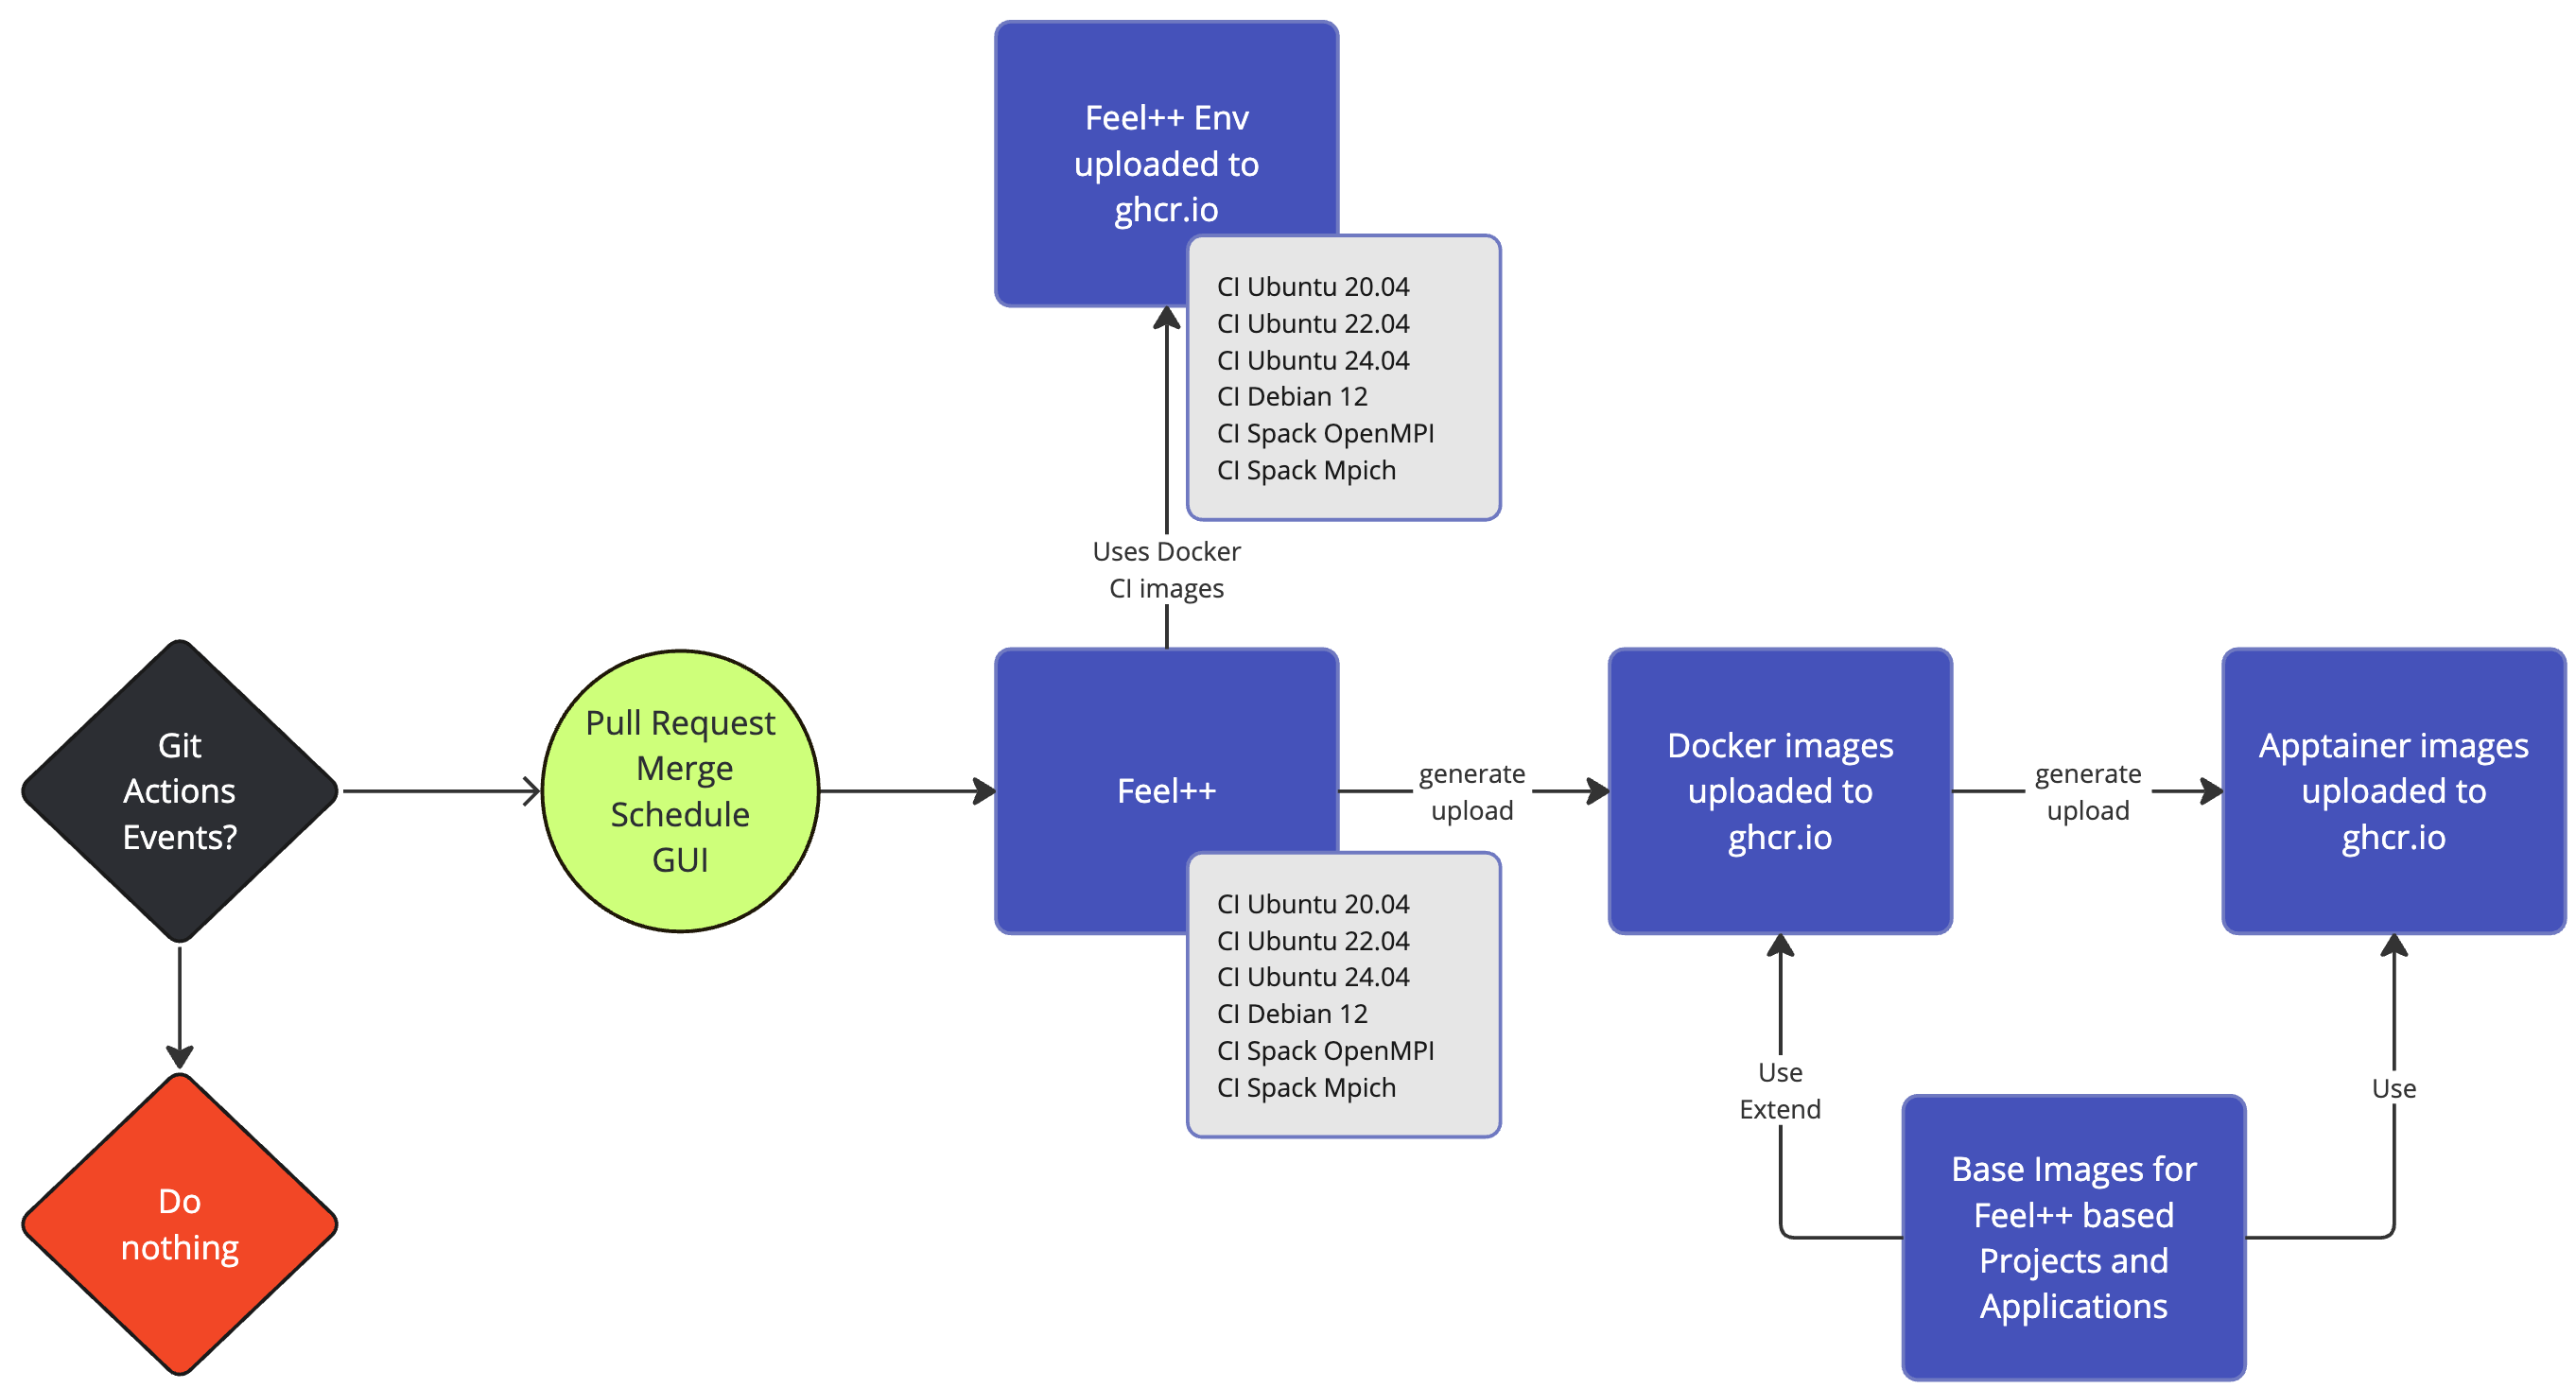
\includegraphics[width=0.8\textwidth]{graphics/feelpp/feelpp-ci-workflow.png}
        \caption{\Feelpp Continuous Integration Workflow using GitHub Actions}
        \label{fig:feelpp-ci}
    \end{figure}

    The~\Cref{fig:feelpp-cb} shows the \Feelpp Continuous Benchmarking Workflow using GitHub Actions and Reframe which is quite close to the methodology described in~\Cref{sec:methodology-regression-reframe}.
    \begin{figure}
        \centering
        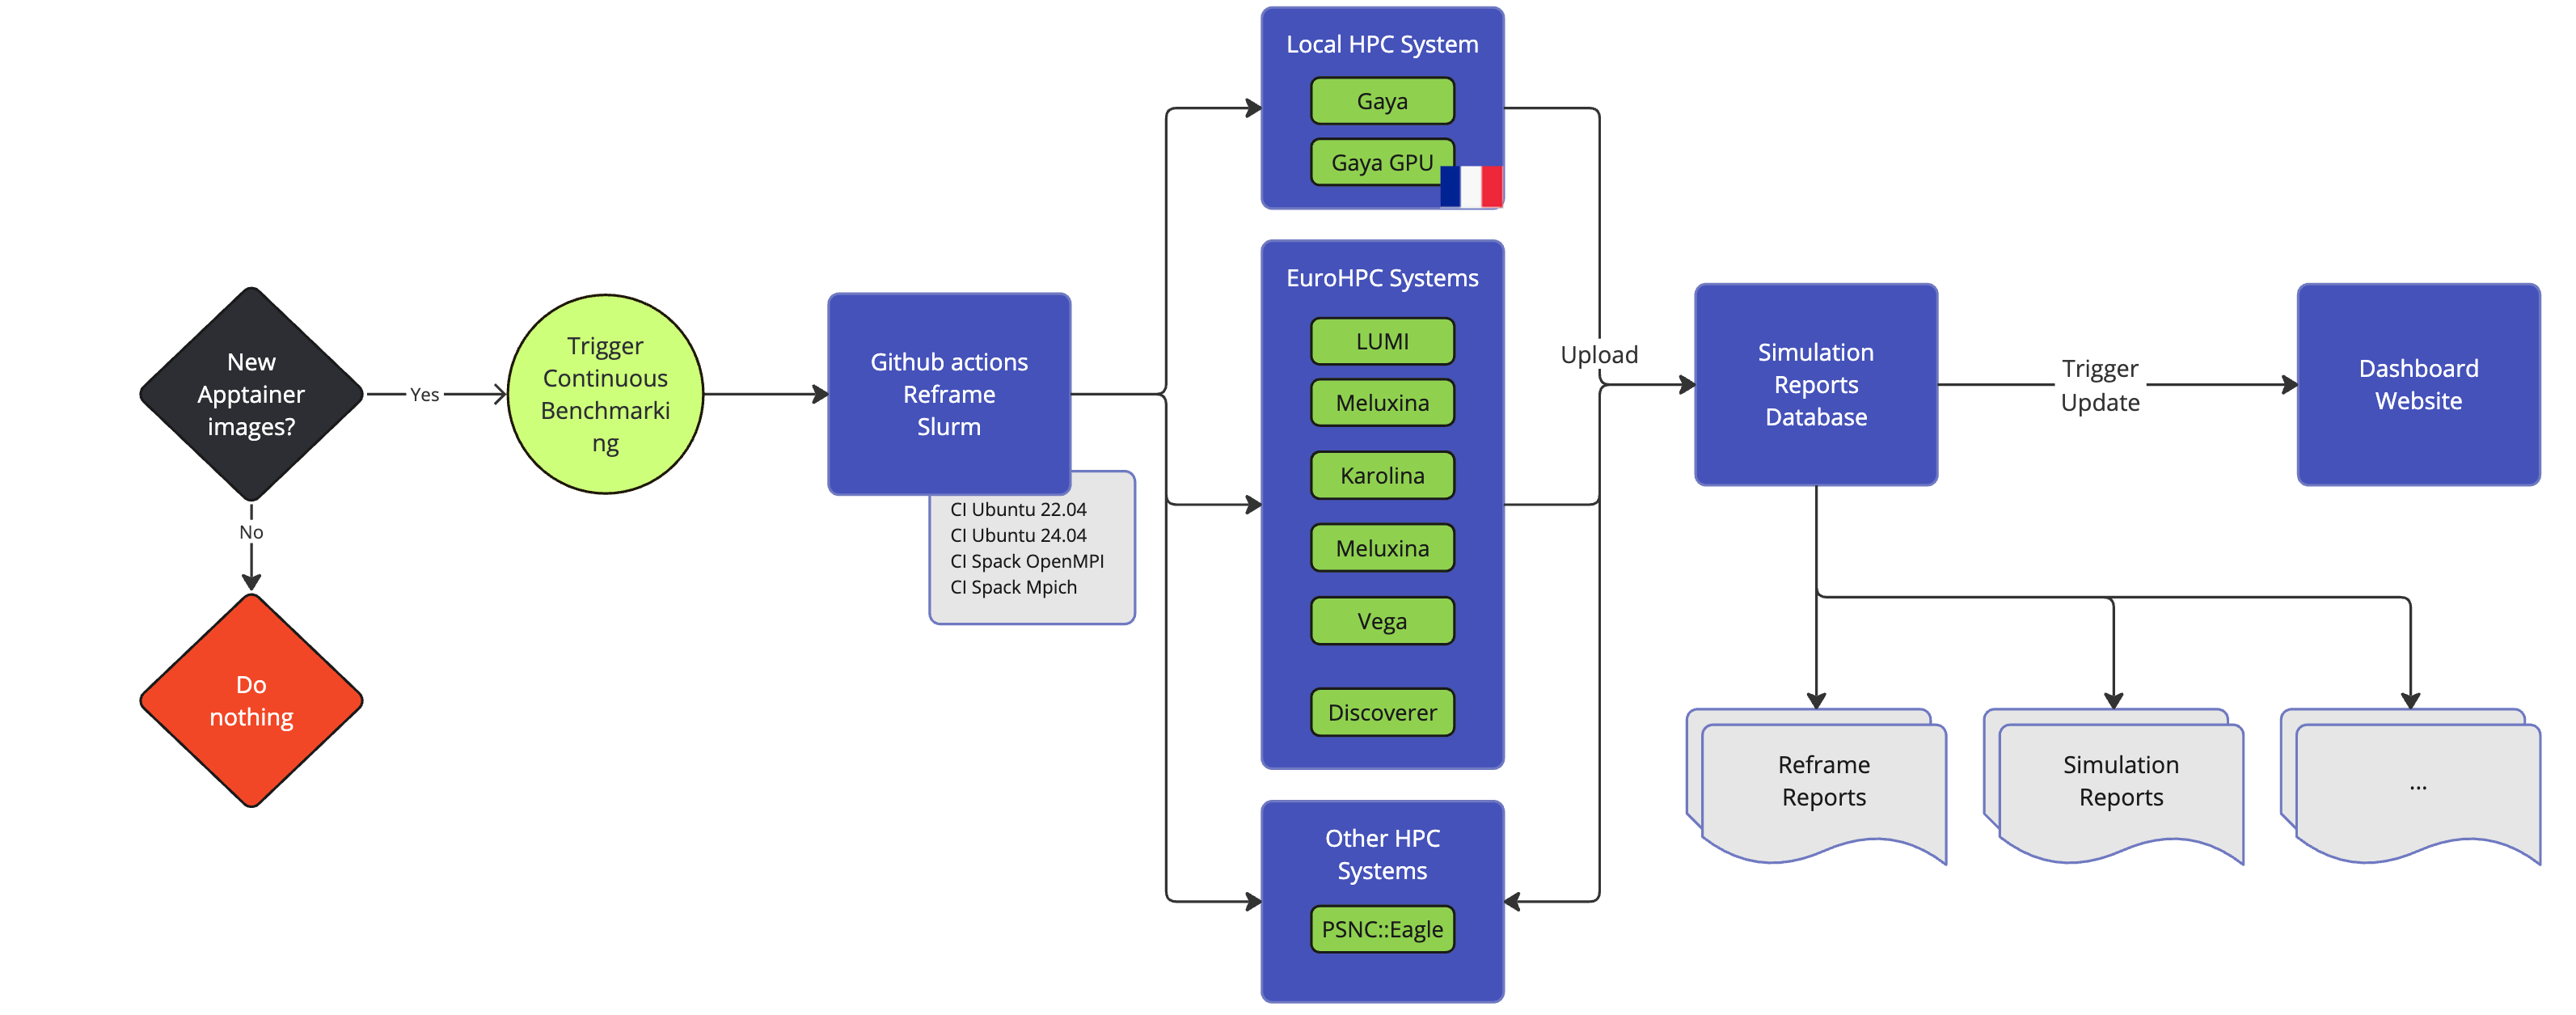
\includegraphics[width=0.8\textwidth]{graphics/feelpp/feelpp-cb-workflow.png}
        \caption{\Feelpp Continuous Benchmarking Workflow using GitHub Actions and Reframe}
        \label{fig:feelpp-cb}
    \end{figure}

\subsection{Mathematics}
\label{sec:Feelpp:mathematics}
\Feelpp is based on the \ac{FEM}, which is used for solving partial differential equations (PDEs) in complex geometries.
It leverages advanced numerical techniques to ensure accuracy and scalability, including adaptive mesh refinement, domain decomposition, and error estimation.

The~\Cref{fig:Feelpp:components} shows the main components of \Feelpp, including the finite element method, mesh generation, solvers but also the components that will be tested in the benchmarks of this deliverable.

\begin{figure}
        \centering
        %!TEX root = ../exa-ma-d7.1.tex

\definecolor{mybluei}{RGB}{70, 82, 186}
\definecolor{myblueii}{RGB}{73,121,193}
\definecolor{mygreen}{RGB}{142, 209, 79}
\definecolor{mypink}{RGB}{255,248,241}

\newcommand\widernode[5][widebox]{
  \node[
    #1,
    fit={(#2) (#3)},
    label=center:{\sffamily\bfseries\color{white}#4}] (#5) {};
}

\begin{tikzpicture}[node distance=3pt,outer sep=0pt,
boxstyle/.style={
  draw=white,
  fill=#1,
  rounded corners,
  font={\sffamily\bfseries\color{white}},
  align=center,
  minimum height=30pt
},
box/.style={
  boxstyle=#1,
  text width=2.5cm},
box/.default=mybluei,
title/.style={font={\sffamily\bfseries\color{white}}},
widebox/.style={draw=white,inner sep=0pt, rounded corners,fill=#1},
widebox/.default=mybluei,
mylabel/.style={font={\sffamily\bfseries\color{white}}},
]

\matrix (stack) [boxstyle=mybluei!40, draw=black,%
        column sep=3pt, row sep=3pt, inner sep=4mm,%
      matrix of nodes,%
        nodes={box, outer sep=0pt, anchor=center, inner sep=3pt},%
        nodes in empty cells,
      %row 1/.style={nodes={fill=none,draw=none,minimum height=3mm}},
]
{
  & & & & \\
& & & & \\  
& & & & \\
& & & & \\
 &  &  &  & Models Description\\
Space Cartesian Products &  & PDE based Preconditioners & Ray-Tracing (BVH) & Level-Set (FastMarching) \\
 & & & &  Forms\\
Finite Elements & Geometric Mapping & & & Export/Import\\
 Timings & & &  &  Quadratures \\
& & & & \\};
\widernode[widebox=mygreen]{stack-1-1}{stack-1-5}{\begin{tabular}{c}Advanced Methods and Analysis:\\ Inverse Problems, Data Assimilation, UQ, ML\ldots \end{tabular}}{Analysis}
\widernode[widebox=mygreen]{stack-2-1}{stack-2-5}{\begin{tabular}{c}Python bindings:\\ Core, \Feelpp Libs, Toolboxes, MOR\end{tabular}}{Python}
\widernode[widebox=mygreen]{stack-3-1}{stack-3-5}{\begin{tabular}{c}ROM: \\RB(Greedy,POD,Error Bounds, SCM/Min-$\theta$, NL-C), (D,G)EIM, PBDW, NIRB\end{tabular}}{RB}
\widernode[widebox=mygreen]{stack-4-1}{stack-4-5}{\begin{tabular}{c}Toolboxes: \\ ALE, CFPDEs, CFD, CSM, Heat, HeatFluid, FSI, ThermoElectric, Maxwell\end{tabular}}{Toolboxes}
\widernode{stack-5-3}{stack-5-4}{Models Description: JSON...}{model}
\widernode{stack-5-1}{stack-5-2}{DSEL for Galerkin Methods}{dsel}
\widernode{stack-6-1}{stack-6-2}{\begin{tabular}{c}Cartesian Products:\\ Spaces, Functions and Forms\end{tabular}}{prod}
\widernode{stack-7-3}{stack-7-4}{Interpolation}{interp}
\widernode{stack-7-1}{stack-7-2}{Function Spaces}{fespace}
\widernode{stack-8-3}{stack-8-3}{Mesh}{Mesh}
\widernode{stack-8-4}{stack-8-4}{Time Discr.}{TimeD}
%\widernode{stack-5-4}{stack-5-5}{Export/Import}{ExImp}
\widernode{stack-9-2}{stack-9-4}{Linear Algebra:
  preconditioner framework, ...}{Alg}
\widernode[widebox=mygreen]{stack-10-1}{stack-10-5}{Core: Environment,
  Logging, Monitoring, Events, Communicators ...}{Core}

\node [fit={(stack.north west)(stack.north
  east)},boxstyle=mybluei!60,draw=black,inner sep=0pt,above=3pt of
stack.north,anchor=south,label={[mylabel]center: Applications: Ktirio Urban Building, Eye2Brain, Swimmer, HifiMagnet}] (AnalysisTools) {};
\node [fit={(stack.south west)(stack.south
  east)},boxstyle=mybluei!60,draw=black,inner sep=0pt,below=3pt of
stack.south,anchor=north,label={[mylabel]center:  Python3, Gmsh, MMG, CGAL, OpenTURNS,  OpenModelica, Salome}] (DepsTools) {};
  \node [fit={(DepsTools.south west)(DepsTools.south
  east)},boxstyle=mybluei!60,draw=black,inner sep=0pt,below=3pt of
DepsTools.south,anchor=north,label={[mylabel]center: C++17, MPI, Boost,
  Google::Glog, MongoDB, Eigen3, PETSc/SLEPc}] (Deps) {};

\end{tikzpicture}

        \caption{Main dependencies of \Feelpp(bottom rows), its main Components as well as the flagship applications (top row).}
        \label{fig:Feelpp:components}
\end{figure}



\subsection{Relevant Publications}
\label{sec:Feelpp:publications}
Relevant publications include:

\begin{description}
        \item[\fullcite{prudhomme_feel_2012}] presents a detailed exploration of \Feelpp's design, focusing on its embedded variational language as a \ac{DSEL} and abstraction mechanisms that simplify the implementation of complex numerical methods. The framework is demonstrated with examples involving non-overlapping domain decomposition techniques and fictitious domain methods.
        \item[\fullcite{prudhomme_feelppfeelpp_2024}] is the last preview of the \Feelpp software. The documentation is available online at \url{https://docs.feelpp.org};
        \item[\fullcite{van_landeghem_mathematical_2024}] The paper \emph{Mathematical and computational framework for moving and colliding rigid bodies in a Newtonian fluid} (2024) presents a mathematical model and computational strategy to simulate the dynamics of moving and colliding rigid bodies within a Newtonian fluid. This work focuses on accurately modeling fluid-structure interactions as a step towards simulating micro-swimmers.
        \item[\fullcite{saigre_model_2024}] The paper \emph{Model Order Reduction and Sensitivity Analysis for Complex Heat Transfer Simulations Inside the Human Eyeball}, presents advanced computational methods to simulate heat transfer processes within the human eye. The authors use reduced-order modeling to improve the efficiency and accuracy of these simulations, contributing to better insights in biomedical engineering through advanced analysis and in particular sensitivity analysis.;
        \item[\fullcite{prudhomme_ktirio_2024}] The paper \emph{Ktirio Urban Building: A Computational Framework for City Energy Simulations Enhanced by CI/CD Innovations on EuroHPC Systems} (2024) presents a high-performance computational framework designed to support the European Union's Horizon 2050 initiative by improving energy consumption in buildings at city scale and beyond. The framework, known as Ktirio Urban Building (KUB), leverages Continuous Integration/Continuous Deployment (CI/CD) innovations to streamline large-scale city energy simulations on EuroHPC JU supercomputers.
        \item[\fullcite{saigre_coupled_2024_abstract}] The paper \emph{A coupled fluid-dynamics-heat transfer model for 3D simulations of the aqueous humor flow in the human eye} presents a coupled fluid-dynamics-heat transfer model to simulate the flow of aqueous humor in the human eye, providing insights into the impact of the postural orientation of the patient on the fluid dynamics and heat transfer processes within the eye. An full-length paper of this extended abstract is in preparation \cite{saigre_coupled_2024_paper}.
        \item[\fullcite{palazzolo2023shape}] The master thesis \emph{Shape Optimization for Rigid Objects in a Stokes Flow} (2023) presents a comprehensive study of shape optimization for rigid objects within a Stokes flow. The research focuses on determining the optimal shapes of 2D and 3D objects using iterative methods, including gradient descent and null-space techniques. The implementation of this work is publicly available at \url{https://feelpp.github.io/feelpp-shapo/shapo/index.html}.
\end{description}

\subsection{Acknowledgements}
\label{sec::Feelpp:acknowledgements}
The software has been developed with the support of the following funding agencies and institutions through various research projects:
\begin{itemize}
   \item Université de Strasbourg
   \item Cemosis
   \item CNRS
   \item ANR
   \item Région Grand Est
   \item AMIES
   \item European Commission
   \item EuroHPC JU
\end{itemize}
